\documentclass[../revisedmain.tex]{subfiles}
\begin{document}
	\vspace{.125in}
	\begin{center}
		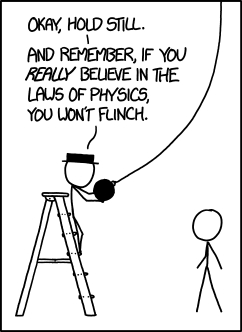
\includegraphics[width=1.5in,height=2in]{physics.png}
	\end{center}
	\vspace{.25in}
The antiderivative is very helpful in physics problems. We already know that $x(t)$, $v(t)$, and $a(t)$ are all related through their rates (derivatives), so they must be related with their antiderivatives as well. There is no single antiderivative for a function, so instead of saying $$\int v(t) dt=x(t)$$ which is false, we can say$$\int v(t)dt=\text{change in }x(t)$$or$$\int v(t)dt=x(t)+C$$At any point $t$, the change in $x(t)$ will be $\int v(t) dt$. This works for all relations as well:$$\int\left(\int a(t) dt\right)dt=\int (v(t)+C)dt=x(t)+Ct+D$$
\end{document}